
\chapter{Introducción}

En la actualidad, los videojuegos se han convertido en el medio de entretenimiento más relevante, no solo a nivel económico, siendo la industria que más ingresos genera \cite{Videojuegos_economia}, sino también a nivel profesional, donde se utilizan como simuladores en el ámbito militar, en la recreación de lugares históricos, entre otros \cite{videojuegos_profesional}. Además, desempeñan un papel clave en el ámbito social, formando grandes comunidades a nivel global. Historias como la de Mats Steen \cite{wow} demuestran que los videojuegos son mucho más que simples programas, ayudando a quienes no están familiarizados con este medio a comprender su impacto y valor.  


También, gracias a la emulación de consolas clásicas, las ofertas diarias, los videojuegos gratuitos, los títulos free-to-play y los servicios de suscripción como Game Pass o PS Plus, es posible acceder a una gran variedad de videojuegos de forma gratuita o a un precio reducido.  


No obstante, el aumento en los costos y recursos necesarios para desarrollar un videojuego \textit{triple A} (término que hace referencia a títulos de gran producción, con una alta inversión en desarrollo y publicidad) ha provocado que los lanzamientos de las sagas más conocidas se espacien cada vez más. Ejemplos de ello son el esperado \textit{Grand Theft Auto VI}, que ha tardado 12 años en llegar desde el lanzamiento de \textit{Grand Theft Auto V}, y \textit{The Elder Scrolls VI}, cuya espera alcanza los más de 14 años desde \textit{The Elder Scrolls V}, según la fecha de realización de este trabajo.  


Debido a esta situación, si queremos disfrutar de experiencias similares a nuestros videojuegos favoritos, a menudo debemos recurrir a entregas anteriores de la misma saga que no jugamos en su momento o bien buscar alternativas en títulos de características similares.  


Algunas plataformas actuales, como Xbox o Steam, recomiendan videojuegos en función de nuestras compras, de los títulos que hemos jugado recientemente o de manera aleatoria. Sin embargo, estas recomendaciones no tienen en cuenta factores importantes, como los recursos de los que disponemos en ese momento, la accesibilidad, el deseo de cambiar de género de videojuego o la disponibilidad de otra plataforma, entre otros.  


A raíz de esta necesidad y como seguidor de este mundillo desde los siete años, se me ocurrió una solución basada en una plataforma capaz de tener en cuenta todos estos aspectos de manera sencilla.  


Parecería que contemplar todos los géneros de videojuegos, sus características y las distintas plataformas es una tarea ardua. No obstante, gracias al avance de la tecnología, contamos con procesadores de lenguaje que han sido entrenados con millones de datos, incluidos videojuegos.  

Si aprovechamos esta tecnología a nuestro favor, podemos obtener fácilmente recomendaciones en tiempo real según los requisitos especificados, utilizando información de consultas previas e incluso teniendo en cuenta los videojuegos que poseemos en nuestra biblioteca, gracias a la vinculación de plataformas de videojuegos con nuestra propia plataforma.  


No debemos limitarnos a usar un solo procesador de lenguaje, sino que es conveniente emplear varios, orquestarlos entre sí y hacer un buen uso de la información previa o de la que se obtiene de manera implícita. Para ello, utilizaremos la novedosa tecnología \textit{LangChain}.  

A lo largo de este trabajo, expondremos qué es esta tecnología, exploraremos sus funciones y revisaremos aplicaciones que la han utilizado, con el objetivo de crear un sistema de recomendación de videojuegos lo más completo, escalable e intuitivo posible.  

\begin{figure}[H]
    \centering
    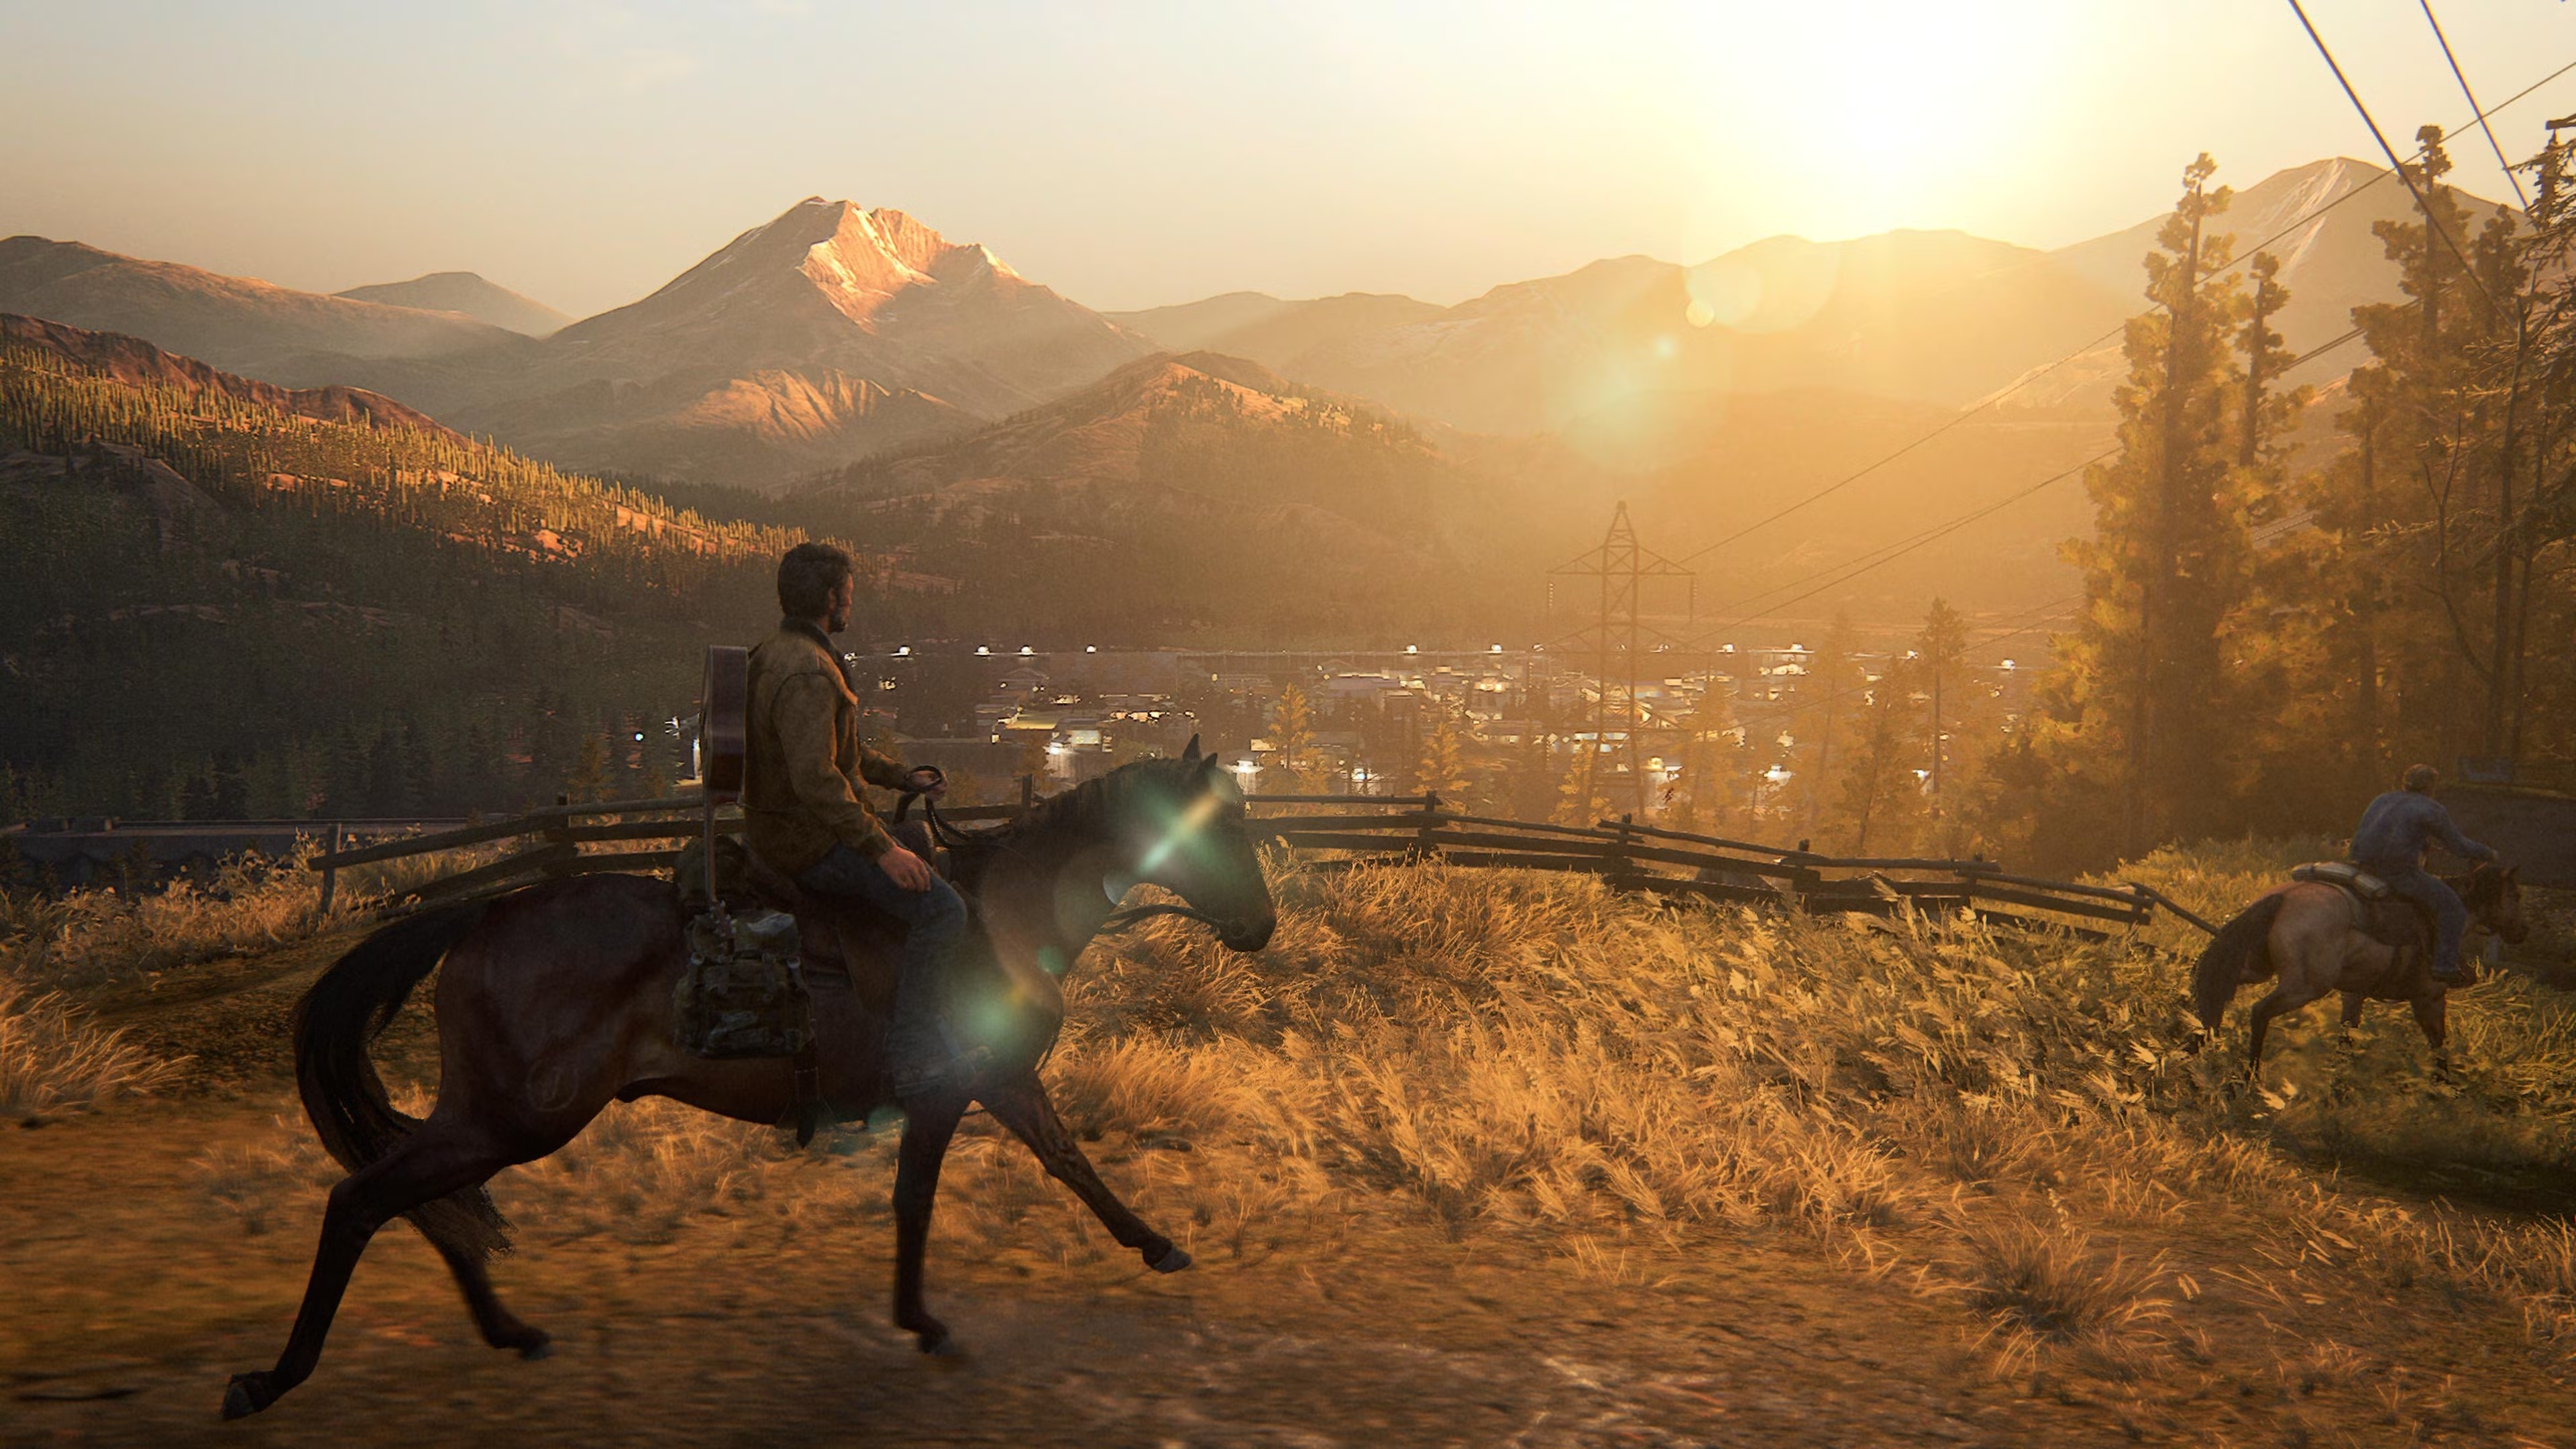
\includegraphics[width=1\linewidth]{imagenes/tlou2.jpg}
    \caption[\textbf{Captura de The Last of Us Parte II}.]{\textbf{Captura de The Last of Us Parte II}, elegido Juego del Año 2020 por los principales medios de la industria. Este videojuego alcanza un nivel gráfico y narrativo sobresaliente. \href{https://static1.srcdn.com/wordpress/wp-content/uploads/2024/01/tlou2r-joel-horse.JPG}{https://static1.srcdn.com/wordpress/wp-content/uploads/2024/01/tlou2r-joel-horse.JPG}}
    \label{foto-the-last-of-us-2}
\end{figure}



